% !TeX root=../main.tex
\chapter{مروری بر کار‌های انجام شده}
\label{LitReview}
%\thispagestyle{empty} 
\section{مقدمه}

مایک هرن\RTLfootnote{\lr{Mike Hearn}}، نویسندهٔ \lr{BIP37} \cite{Hearn2013}
در پست \cite{Hearn2015} خودش اعلام می‌کند که فیلتر بلوم از امنیت کافی برخوردار نیست. او در این پست به برخی از ایراداتی که در بخش \ref{Vulnerabilities} به آن‌ها اشاره شده، پرداخته است. همچنین مروری بر راه‌حل‌های جایگزین از جمله استفاده از روش‌های بازیابی اطلاعات خصوصی\RTLfootnote{\lr{Private Information Retrieval (PIR)}}
(PIR)
، رمزنگاری ارتباط همتا‌به‌همتا برای جلو گیری از افشا شدن اطلاعات نزد طرف‌های متخاصم، از جمله سازمان‌های اطلاعاتی، اشاره می‌کند. هرن همچنین توضیح می‌دهد که حل این مسئله ساده نخواهد بود و به دشواری‌ها و چالش‌های آن اشاره کرده است\cite{Hearn2015}.

علاوه بر این، افراد دیگری پیشنهاد‌های زیادی در تغییر شیوهٔ موجود ارائه کرده‌اند که در این قسمت به بررسی پیشنهاد‌ها و راه‌حل‌هایی که تا کنون برای بهبود حریم خصوصی کاربران سبک منتشر است پرداخته می‌شود. 


\subsection{
اصلاح رفتار کاربر سبک فعلی جهت حفظ حریم خصوصیش
}
\label{change_behaviour}
در مقالهٔ \cite{Gervais2014} در کنار تحلیل امنیت و بیان ضعف‌های استفاده از فیلتر بلوم در ارتباط بین گره سبک با گره کامل \cite{Hearn2013}، به بیان چند رویه پرداخته است که اگر گره سبک از این رویه‌ها پیروی کند، می‌تواند در عین این که از پروتکل فعلی استفاده می‌کند، تا حدی حریم خصوصی خودش را حفظ کند. در ادامه به بیان این موارد پرداخته می‌شود.

	همان‌طور که در \ref{Vulnerabilities} نشان داده شد، نرخ خطای نوع دوی فیلتر بلوم به طور قابل ملاحظه‌ای تحت تاثیر تعداد عناصر قرار گرفته در یک فیلتر بلوم است. همچنین باید از ایجاد چند فیلتر بلوم با عناصر مشترک پرهیز شود. در نتیجه پیشنهاد می‌شود هر گره سبک در ابتدا یک فیلتر بلوم با $N$ آدرس ایجاد کند به طوری که $M=N$. به این ترتیب، فیلتر بلوم با نرخ خطای نوع دوی هدف، $P_t$، ساخته می‌شود. همچنین پیشنهاد شده است که $M=m$، به این معنی که تنها یکی از مقادیر \lr{PubKey} یا \lr{PubKeyHash} در فیلتر بلوم قرار بگیرد. مقالهٔ \cite{Gervais2014} بررسی کرده است که برای تقریبا $99\%$ از آدرس‌های بیت‌کوین قرار دادن یکی از این دو مقدار در فیلتر بلوم کفایت می‌کند تا تمام تراکنش‌های مرتبط  با خودشان را دریافت نمایند.
	
	گره سبک می‌تواند به مرور که به آدرس‌های بیشتری نیاز پیدا کرد، از $N$ آدرسی که پیش‌پیش در فیلتر بلوم قرار گرفته است، استفاده نماید. زمانی که از تمام این $N$ آدرس استفاده کرد، یک فیلتر بلوم جدید تولید نماید که این هم شامل $N$ آدرس جدید باشد و آدرس مشترکی با فیلتر بلوم قبلی نداشته باشد. گره سبک می‌تواند این که هر آدرسش در کدام فیلتر بلوم قرار گرفته‌ است را تحت اطلاعاتی جانبی، در کنار آدرس‌هایش، ذخیره نماید. در این صورت گره متخاصم نمی‌تواند با در دست داشتن فیلتر‌های بلوم مربوط به یک کیف پول به اطلاعات اضافه‌ای دست پیدا کند. به این ترتیب گره سبک باید همزمان از چند فیلتر بلوم استفاده نماید و آن‌ها را برای گره‌های مختلف ارسال کند. البته خود مقالهٔ \cite{Gervais2014} اذعان داشته است که در صورتی که گره سبک برای اولین بار از یک آدرس از پیش ذخیره شده در فیلتر بلوم استفاده نماید، از آن‌جایی که این آدرس تا الان در زنجیره بلوکی استفاده نشده است و در اولین استفاده‌اش با فیلتر بلوم این کاربر منطبق شده است، می‌تواند گره کامل را مطمئن سازد که این آدرس جزء آدرس‌های اصلی این فیلتر بلوم است.
	
	برای حفظ بیشتر حریم خصوصی کاربر و رفع ضعف ذکر شده، مقالهٔ \cite{Gervais2014} پیشنهاد داده است که گره سبک با توجه به آدرس‌های موجود در زنجیرهٔ بلوکی، که مربوط به خودش نیستند، دست به ایجاد یک فیلتر بلوم بزند. سپس سعی کند برای هر آدرسی که احتیاج دارد، با تلاش‌ها و آزمون‌ و خطا‌های مکرر آدرس جدید را طوری ایجاد نماید که در فیلتر بلوم تولید شده قرار گیرد. در نتیجه در صورت قرار گرفتن آدرس تازه ساخته شدهٔ این گره در زنجیرهٔ بلوکی، احتمال بیشتری وجود خواهد داشت که گره کامل آن تراکنش آن را برای گره‌های دیگری نیز ارسال نماید. اما این روش بار پردازشی زیادی را بر روی گره سبک بابت تولید آدرس جدید تحمیل می‌کند.  
	
در هر بار راه‌اندازی یک کیف پول در یک گره سبک، نرم‌افزار کیف پول شروع به محاسبهٔ مجدد فیلتر بلوم با استفاده از آدرس‌هایش می‌نماید چرا که فیلتر بلوم تولید شده‌اش را در حافظه دائمی ذخیره نمی‌کند. در نتیجه، این موضوع می‌تواند باعث شود که فیلتر‌های بلوم متعددی با $nTweak$های متفاوت اما عناصر یکسان در دست یک گره کامل بیافتد. مقالهٔ \cite{Gervais2014} پیشنهاد داده است که گره سبک فیلتر بلومش و اطلاعات جانبی آن مانند آدرس‌هایی که در آن قرار گرفته است و غیره را در یک حافظهٔ دائمی ذخیره کند. این مقاله تخمین زده است که هر گره سبک نیاز خواهد داشت که برای هر فیلتر بلوم، چیزی در حدود $220$ بایت ذخیره نماید که سربار قابل توجهی به نرم‌افزار کیف پول اضافه نمی‌کند.
	
	روش‌های پیشنهاد شده در این قسمت، هر چند تا حدودی توانسته بودند ضعف‌های اساسی \cite{Hearn2013} را جبران نمایند، اما به طور کامل نتوانسته بودند که ایرادات آن را برطرف کنند.  علاوه بر این، روش‌های پیشنهاد شده نسبت به حملهٔ تحلیل بسامد پرسمان و استفاده، آسیب پذیر است. همچنین راه حل مشخصی  پیشنهاد نشده است که جلوی گره کامل متخاصم گرفته شود تا نتواند از روی روابط بین آدرس‌های یک فیلتر بلوم به آدرس‌های اصلی پی ببرد. باید به این نکته نیز توجه کرد که یکی از دلایلی که در پیاده‌سازی گره سبک، المان‌های فیلتر تازه ساخته شده باتوجه به $M=m+100$ بوده است آن است که اجازهٔ به روزرسانی فیلتر با توجه به تراکنش‌های منتشر شده در شبکه، طبق جدول \ref{table:filterloadMessage}، به گره کامل داده شود و در عین حال جلوی اشباع زودهنگام فیلتر گرفته شود. اما با توجه به راه حل \cite{Gervais2014}، که پیشنهاد داده است که در همان ابتدا $M=m$ باشد، امکان به روزرسانی فیلتر با توجه به تراکنش‌های جدید سلب می‌شود.


\subsection{معیار 
	حاشاپذیری-$\gamma$ برای
	سنجش حریم خصوصی فیلتر بلوم}
\label{gamma-deniability}

در مقاله \cite{Bianchi2012} معیاری کمّی، بر اساس مدل گمنامی-$K$ 
\cite{Sweeney2002}،
برای اندازه‌گیری حریم خصوصی فیلتر بلوم معرفی شده است. در این مقاله بیان شده است که احتمال خطای نوع دو ($P_f$) به تنهایی معیار مناسبی برای سنجش حریم خصوصی فیلتر بلوم نیست. بلکه باید تعداد عناصر خطای نوع دو ($N_v$) مورد بررسی قرار گیرد. واضح است که اندازهٔ $N_v$ علاوه بر $P_f$ وابسته به تعداد کل عناصر ($N_u$) است:
$N_v=(N_u-m)\times P_f$.
با توجه به این موضوع، مقاله \cite{Bianchi2012} با بهره‌برداری از نسخهٔ احتمالاتیِ مدل گمنامی-$K$
\cite{Lodha2008}،
یک معیار سنجش گم‌نامی مناسب فیلتر بلوم ارائه داده است. عنوان این معیار «حاشاپذیری-$\gamma$» است. 

در فیلتر بلوم، داده به صورت تجزیه ناپذیر ذخیره می‌شود و در گمنامی-$K$ داده به صورت ساختاریافته و دارای ویژگی‌های مشخصی هست. اما می‌توان شباهت‌های نزدیکی بین آن‌ها در نظر گرفت. به طور شهودی می‌توان این گونه تعبیر کرد که بیت‌های فیلتر ($b[i]$ و $i\in[0,n-1]$) «ویژگی‌های» عنصر $x$ هستند. یعنی، عنصر $x$ دارای ویژگی $b[i]$ است، اگر و تنها اگر به ازای حداقل یک 
$j\in[1,k]$ داشته باشیم 
$H_j(x)=i$.
به این ترتیب می‌توانیم از تعریف گمنامی-$K$ در فیلتر بلوم استفاده نماییم. عنصر $x$، قرار گرفته در فیلتر، گمنام-$K$ یقینی است اگر به ازای تمام بیت‌های $b[i]$  که توسط این عنصر یک شده‌اند، حداقل $K-1$ عنصر خطای نوع دو وجود داشته باشد که به همان بیت‌ها نگاشت شوند.

می‌توان از این تعریف فهمید که برقراری شرایط گمنامی-$K$ یقینی همیشه امکان‌پذیر نیست. از این رو، استفاده از تعمیم احتمالاتی گمنامی-$K$ 
\cite{Lodha2008} 
برای فیلتر بلوم مناسب‌تر است. به این ترتیب مقالهٔ \cite{Bianchi2012} برای عنصری که به فیلتر بلوم اضافه شده است، از صفت «حاشاپذیر» استفاده کرده است.  به این معنی که آیا دارنده فیتلر می‌تواند وجود آن عنصر در فیلتر را انکار نماید یا خیر. به این ترتیب می‌گوییم عنصر $x\in \mathcal{S}$ حاشاپذیر است اگر به ازای 
$\forall i \in \{1..k\}$،
حداقل یک عنصر از مجموعه پنهان‌سازی $v\in \mathcal{V}$ (خطای نوع دو) وجود داشته باشد به گونه‌ای که 
$\exists j \in \{1..k\}$
به شرطی که 
$H_i(x) = H_j(v)$.
به بیان ساده‌تر یک عنصر حاشا‌پذیر است اگر بتوان بدون تغییر بیت‌های فیلتر، آن عنصر را توسط عناصری که عضو فیلتر نیستند جایگذاری کرد. 

فیلتر بلوم $B$، حاشاپذیر-$\gamma$ است (یا دارای ویژگی حاشاپذیری-$\gamma$) است، هر گاه یک عنصر تصادفی آن $x\in \mathcal{S}$ با احتمال $\gamma$ حاشاپذیر باشد. احتمال تقریبی حاشاپذیری-$\gamma$ فیلتر $B$ به صورت معادله \eqref{eq:gamma-deniability} محاسبه می‌شود  \cite{Bianchi2012}.

\begin{equation}
\gamma \left(B\right) \approx \left(1-exp\left(-\frac{N_vk}{n\left(1-e^{-km/n}\right)}\right)\right)^k
\label{eq:gamma-deniability}
\end{equation}

که در آن 
$N_v=(N_u-m)\times P_f$.
هرچه مقدار $\gamma$ به یک نزدیک‌تر باشد، سطح بهتری از حریم خصوصی مُهیا شده است.
شکل \ref{fig:gamma_deniability} مثالی را نشان می‌دهد که در آن   
$\mathcal{S} = \{x_1, x_2, x_3\}$ 
مجموعه عضو فیلتر بلوم است. مجموعهٔ پنهان‌سازی (خطای نوع دو)، شامل عناصر 
$\mathcal{V} = \{v_1, v_2, v_3\}$
می‌شود. عنصر $x_1$ حاشا‌پذیر است چرا که بیت‌های مرتبط با آن، یعنی $b[0]$، $b[2]$ و $b[7]$، توسط عناصر $v_1$ و $v_2$ پوشانده شده است. به همین ترتیب می‌توان نشان داد که عنصر $x_2$ نیز حاشا‌پذیر است. اما عنصر $x_3$ حاشا‌پذیر نیست. چرا که بیت $b[8]$ توسط هیچ‌کدام از عناصر مجموعهٔ پنهان‌سازی پوشانده نشده است. به این ترتیب، این فیلتر به صورت کلی، حاشاپذیر-$0.66$ است.


\begin{figure}
	\centering
	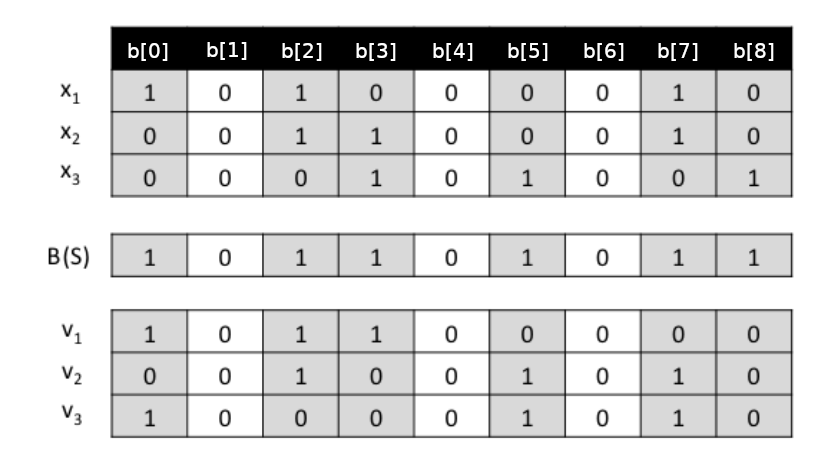
\includegraphics[width=0.8\linewidth]{image/gamma_deniability}
	\caption[مثالی از حاشاپذیری-$\gamma$]{
		یک فیلتر بلوم تشکیل شده از عناصر $\{x_1, x_2, x_3\}$ که سه عنصر $\{v_1, v_2, v_3\}$ را به عنوان خطای نوع دو می‌پذیرد\cite{Bianchi2012}.
		
	}
	\label{fig:gamma_deniability}
\end{figure}

در \cite{Kanemura2017} پیشنهاد شده است که فیلتر بلوم استفاده شده در پروتکل بیت‌کوین با توجه به معیار حاشاپذیری-$\gamma$  
\cite{Bianchi2012}،
ساخته شود. زیرا نرخ خطای نوع دو ($P_t$) به تنهایی برای سنجش حریم خصوصی فیلتر بلوم ساخته شده کافی نیست. به این ترتیب لازم است که طبق معادله \eqref{eq:gamma-deniability} در هر لحظه باتوجه به تعداد آدرس‌های یکتایی که از نقطه بررسی تا آخرین بلوک استخراج شده در زنجیره بلوکی نمایان شده‌اند ($N_u$) و $\gamma$، مقدار $P_t$ تعیین گردد. از آن‌جایی که محاسبه $N_u$ برای گره سبک غیرممکن است، در \cite{Kanemura2017} پیشنهاد شده است که از تکنیک رگرسیون خطی برای تخمین  $N_u$  استفاده شود. ضرایب مدل رگرسیون خطی، باید متناوبا (مثلا به صورت هفتگی) محاسبه گردد. این محاسبه می‌تواند به توسعه دهندگان نرم‌افزار که طرح ارائه شده در \cite{Kanemura2017}  را پیاده‌سازی می‌کنند، سپرده شود. به این ترتیب گره سبک می‌تواند مقدار $P_t$ را به نحوی تعیین کند که از امنیت فیلتر بلوم مطمئن گردد.

روش ارائه شده در \cite{Kanemura2017} دارای اشکالاتی است. یکی از اصلی‌ترین این اشکالات به روزرسانی متناوب فیلتر بلوم باتوجه به تخمین حاصل از $N_u$  است. طبق مقاله \cite{Gervais2014}، اگر گره کامل متخاصم به دو فیتلر بلوم که مربوط به یک گره سبک هستند دست پیدا کند، می‌تواند با دقت بیش‌تری آدرس‌های مربوط به گره سبک را حدس بزند. از این رو تولید متناوب فیلتر بلوم می‌تواند حریم خصوصی کاربر سبک را به خطر بیاندازد.
از ایرادات دیگر این روش می‌توان به افزایش $P_t$ در نتیجهٔ به کار گیری از این طرح اشاره نمود. به این ترتیب، پهنای باند مورد نیاز زیادتر می‌شود. 

\subsection{فیلترکردن بلوک}
\label{BIP157}
در \cite{Osuntokun2017} پیشنهاد شده است که بر خلاف آن‌که گره سبک فیلتر بلوم را تولید کند و برای گره کامل ارسال نماید، گره کامل یک فیلتر از روی تمام دادگان یک بلوک ایجاد ‌کند. گره سبک به ازای هر بلوک جدید، فیلتر مربوطه را از گره کامل دریافت کرده و خودش بررسی می‌کند که آیا داده مورد نظرش در آن قرار دارد یا نه. اگر داده مورد نظر گره سبک در آن فیلتر قرار داشت، تمام بلوک را از گره کامل دریافت می‌کند. این ایده برای اولین بار در ایمیل آدام بک\RTLfootnote{\lr{Adam Back}}، از دانشمندان حوزهٔ بیت‌کوین، بیان شده است\cite{Back2015}. به فیلتر استفاده شده در این روش 
فیلتر بلوک\RTLfootnote{\lr{Block Filter}}
 گفته می‌شود. کیف پول 
 نوترینو\RTLfootnote{Neutrino}
در حال حاضر از این روش پشتیبانی می‌کند.

از آن‌جایی که مقدار ساخته شده برای فیلتر‌ها یقینی هستند، نیاز است تنها یک مرتبه ساخته شده و ذخیره شوند. بر خلاف فیلتر بلوم، در این روش از یک عدد تصادفی برای ساخت فیلتر استفاده نمی‌شود. از این رو گره کامل از خطر حملات منع خدمت در امان است. در این روش برای هر فیلتر بلوک یک سرایند مرتبط وجود دارد که اندازهٔ این سرایند $32$ بایت بوده و سرایند شامل چکیدهٔ مقدار حاصل از 
الحاق\RTLfootnote{Concatenate} چکیدهٔ فیلتر بلوک و سرایند فیلتر بلوک قبلی است. سرایند فیلتر بلوک برای هر بلوک زنجیرهٔ قالبی می‌تواند به عنوان یک خروجی \lr{\texttt{OP\_RETURN}} در تراکنش کوین‌بِیس\RTLfootnote{ \lr{Coinbase}} قرار بگیرد. 

در این روش، هر فیلتر بلوک به ازای هر تراکنش‌ بلوک شامل نبشتهٔ‌های خروجی قبلی که در هر ورودی‌ آن خرج شده است می‌شود همچنین تمام \lr{scriptPubKey}های هر خروجی تمام تراکنش‌ها نیز در آن قرار می‌گیرد. در این روش نیز اگر عنصری در فیلتر قرار گرفته باشد، با احتمال 1 در آن صدق می‌کند اگر قرار نداشته باشد با احتمال $\frac{1}{M}$ با آن منطبق می‌شود. مراحل ساخت فیلتر بلوک با \lr{N} عضو، به شرح زیر است (توجه شود که
$N,M < 2^{32}$)
\begin{enumerate}
	\item {%
	چکیدهٔ تمام اعضای فیلتر بلوک با استفاده از تابع چکیده‌ساز \lr{SipHash} محاسبه می‌شود. سپس خروجی تابع چکیده‌ساز به صورت یکنواخت در بازهٔ 
	$[0, N\times M)$
	نگاشت می‌شود. 
}

\item {%
	مقادیر خروجی مرحلهٔ قبل با توجه به مقدارشان مرتب می‌شوند و اختلاف هر دو مقدار متوالی محاسبه می‌شود. برای کوچک‌ترین مقدار، اختلاف آن با صفر محاسبه می‌شود که برابر با خودش است.
 }

\item {%
مقادیر اختلاف‌ها که از مرحلهٔ قبل بدست آمده پشت سر هم نوشته می‌شوند و به وسیلهٔ کدگذاری گلومب-رایس\RTLfootnote{\lr{Golomb-Rice coding}} فشرده می‌شوند.
}

\end{enumerate}

از آن‌جا که خروجی مرحلهٔ یک دارای یک توزیع یکنواخت\RTLfootnote{\lr{Uniform distribution}} است،‌ اخلاف آن‌ها دارای یک توزیع هندسی\RTLfootnote{\lr{Geometric distribution}} خواهد بود. روش کدگذاری گلومب-رایس در فشرده‌سازی داده‌هایی با توزیع هندسی بهینه عمل می‌کند\cite{Osuntokun2-2017}. برای کدگذاری گلومب-رایس، شپارامتر $P$ تعریف می‌شود که طول کد باقیمانده را تعیین می‌کند. این کد‌گذاری به این صورت است که هر مقداری (در اینجا اختلاف بین دو چکیده) بر $2^P$ تقسیم شده و خروجی آن دو قسمت خارج قسمت $q$ و باقیماندهٔ $r$ خواهد بود. سپس، $q$ با روش کدگذاری یگانی\RTLfootnote{\lr{Unary coding}}، که به صورت رشته‌ای خواهد بود که با تعداد $q$ یک به همراه یک $0$ نوشته می‌شود. مقدار $r$ هم در $P$ بیت با استاندارد اندین بزرگ نوشته می‌شود. به عنوان مثال کدگذاری عدد $9$ با $P=2$  به صورت
 \lr{\texttt{110 01}} 
 خواهد بود. که در آن $q=2$ و $r=1$ است.
 
 در این روش امکان استفاده از فیلتر‌های مختلف وجود دارد اما در فیلتر اولیهٔ این روش، مقدار $M=784931$ و مقدار $P=19$ است. حال در این پایان‌نامه، برای آن‌که تخمینی از سربار پهنای باندی برای گره سبک در این روش داشته باشیم، به این ترتیب عمل می‌کنیم:
 \begin{itemize}
 	\item {%
 در زمان نگارش این پایان‌نامه، تعداد روزانهٔ هرکدام از ورودی‌ها و خروجی‌های \lr{P2PKH} حدودا برابر $350,000$ عدد است\RTLfootnote{\lr{\url{https://transactionfee.info/charts/inputs-and-outputs-p2pkh/}}} که در مجموع می‌شود $700,000$ عدد در روز. همچنین برای \lr{P2SH}، تعداد خروجی‌ها برابر $310,000$ و تعداد ورودی‌ها برابر $22,000$عدد است\RTLfootnote{\lr{\url{https://transactionfee.info/charts/inputs-and-outputs-p2sh/}}}
 که در مجموع تعداد آن برابر $332,000$ عدد در روز خواهد بود.
به این ترتیب برای هر هر فیلتر بلوک در زمان نگارش پایان‌نامه می‌توان $7167$ عضو متصور شد($N=7167$)
}
\item{%
با فرض اینکه از فیلتر اولیه استفاده شود، $M=784931$ و $P=19$ خواهد بود. به این ترتیب از آن‌‌جا که خروجی چکیدهٔ اعضای فیلتر بلوک، در بازهٔ 
$[0, N\times M)$
نگاشت می‌شوند، نتایج در بازهٔ صفر تا 
$N\times M = 5,625,600,477$
به صورت یک‌نواخت توزیع خواهد شد.\\
\begin{equation}
\label{eq:Items_in_block_filter}
0\le h_1 \leq h_2 \leq \dots \leq h_N < 5.625 \times 10^{9}
\end{equation}
که در آن $h_i$ها خروجی تابع چکیده‌ساز بعد از نگاشت به بازهٔ گفته شده بوده که به ترتیب اندازهٔ آن‌ها مرتب شده‌اند.
}
\item{%
با توجه به روش گفته شده تفاضل بین $h_i$ها را به صورت زیر محاسبه می‌کنیم:
\begin{equation}
\label{eq:delta_value_in_block_filter}
\delta_i = h_i - h_{i-1}, \ \  1<i\leq N; \quad \delta_1 = h_1
\end{equation}
}
\item{%
حال باید بر روی مقادیر $ \delta_i $ کدگذاری گلومب-رایس اعمال شود و بیت‌های حاصل به ترتیب در کنار هم قرار بگیرند. تعداد بیت‌های خروجی برای یک فیلتر بلوک ($L$) از فرمول زیر محاسبه می‌شود.



\begin{multline}
\label{eq:size_in_block_filter}
L = \sum_{i=1}^{N} \left(\left[\frac{\delta_i}{2^P}\right] + P + 1\right) < \\
\left[\frac{\sum_{i=1}^{N} \delta_i }{2^P}\right] + NP + N  <
\left[\frac{ MN }{2^P}\right] + N(P + 1) 
\end{multline}

که در آن 
$\frac{\delta_i}{2^P}$
تعداد یک‌های حاصل از کدگذاری هر کدام از 
$\delta_i$ها
است و به ازای هر کدام از آن‌ها یک بیت صفر و $P$ بیت شامل باقیمانده قرار داده می‌شود. مجموع تفاضل‌های $ \delta_i $ برابر با $h_N$ می‌شود و با توجه به \eqref{eq:Items_in_block_filter}، این مقدار می‌تواند حداکثر $MN$ باشد.

}
%\item{%
%با توجه به معادلهٔ \eqref{eq:Items_in_block_filter}، و اینکه $h_i$ها توزیع یکنواخت دارند. می‌خواهیم $E\{L\}$ را محاسبه کنیم. 
%\begin{equation}
%\label{eq:E_L_1_block_filter}
%E\{L\} \approx \left[\frac{E\{h_N\}}{2^P}\right] + NP + N
%\end{equation}
%
%که با توجه به \eqref{eq:Items_in_block_filter} و استقلال $h_i$ها ، برای محاسبهٔ $E\{h_N\}$ داریم:
%\begin{equation}
%\label{eq:E_h_N_1_block_filter}
%F_{h_N}(x) = \left[F_{h}(x)\right]^N
%\end{equation}
%
%و از آن‌جایی که توزیع $h$ یکنواخت در بازهٔ 
%$[0, NM)$
%است، خواهیم داشت:
%\begin{align}
%\label{eq:E_h_block_filter}
%F_{h}(x) = \frac{x}{N M} \qquad \text{for} \quad  0 \leq x < NM\\
%\Rightarrow F_{h_N}(x) = \frac{x^N}{(NM)^N} \qquad \text{for} \quad  0 \leq x < NM\\
%\Rightarrow f_{h_N}(x) = \frac{Nx^{N-1}}{(NM)^N} \qquad \text{for} \quad  0 \leq x < NM
%\end{align}
%
%به این ترتیب:
%
%\begin{multline}
%\label{E_h_2_block_filter}
%E\{h_N\} = \int_{0}^{NM} xf_{h_N}(x) dx \\
%= \int_{0}^{NM} \frac{Nx^{N}}{(NM)^N} = \frac{N}{(NM)^N} \cdot \left. \frac{x^{N+1}}{N+1} \right|_0^{NM} = \frac{N^2M}{N+1} \approx NM
%\end{multline}
%
% 
%که با توجه به معادلهٔ بالا و \eqref{eq:E_L_1_block_filter} داریم:
%\begin{equation}
%\label{E_L_2_block_filter}
%E\{L\} \approx \left[\frac{NM}{2^P}\right] + (N+1)P
%\end{equation}
%با توجه به مقادیر $N$، $M$ و $P$ داریم:
%
%\begin{equation}
%\label{E_L_3_block_filter}
%E\{L\} \approx \left[\frac{5.625 \times 10^{9}}{2^{19}}\right] + 7168 \times 19 = 146921\text{b} = 18366\text{B} = 18\text{KB}
%\end{equation}
%
%
%}

\item{%
با توجه به مقادیر $N$، $M$ و $P$ داریم:

\begin{equation}
\label{E_L_3_block_filter}
L < \left[\frac{5.625 \times 10^{9}}{2^{19}}\right] + 7168 \times 19 = 146921\text{b} = 18366\text{B} = 18\text{KB}
\end{equation}


}
 \end{itemize}

به این ترتیب می‌توان گفت که اندازهٔ هر فیلتر بلوک از $18$ کیلوبایت کوچک‌تر است. با توجه به زیاد بودن اندازهٔ $M$، احتمال آن‌که یک بلوک به عنوان خطای نوع دو انتخاب شود بسیار کم خواهد بود. هرچند که کم بودن نرخ خطای نوع دو باعث کاهش پهنای باند مصرفی گره سبک می‌گردد، اما از طرف دیگر می‌تواند حریم خصوصی کاربر سبک را با خطر مواجه کند.

اگر گره سبک از آدرس‌های محدودی استفاده کند به گره کامل متخاصم این امکان را می‌دهد که بتواند با در نظر گرفتن آدرس‌های مشترک بین بلوک‌های درخواست شده توسط آن کاربر، آدرس کاربر را در مجموعه محدود‌تری جست‌وجو نماید. گره کامل با استفاده از گراف تراکنش‌ها حتی می‌تواند به نتایج دقیق‌تری دست پیدا کند\cite{blockfilter-wiki}.

مشکل دیگر این روش، کاربرد آن برای گره‌های سبکی است که تراکنش‌های نسبتا زیادی در شبکه ارسال می‌کنند. حریم خصوصی این گره‌ها نه تنها بیش‌تر در معرض نقض شدن قرار دارد، بلکه، آن‌ها برای هم‌گام سازی با شبکه نیاز است که پهنای باند زیادی را مصرف نمایند. چرا که لازم است برای هر تراکنش، یک بلوک کامل را دانلود نمایند.

گره کامل متخاصم می‌تواند با تحلیل‌ بسامد درخواست‌ها و آدرس‌های بلوک درخواست داده شده تعدادی از آدرس‌های پوششی بلوک‌های درخواست داده شده را کنار بگذارد و در مجموعهٔ کوچک‌تری به جست‌و‌جوی آدرس‌‌های کاربر سبک بپردازد.

\subsection{بازیابی اطلاعات خصوصی}
\label{PIR}
در مقاله \cite{Qin2019} از روش بازیابی اطلاعات خصوصی (PIR) جهت دریافت اطلاعات تراکنش‌ها از گره‌ کامل استفاده کرده است. بازیابی اطلاعات خصوصی به کاربران این امکان را می‌دهد که از یک پایگاه داده یا مجموعه‌ای از آن‌ها یک پرسمان انجام دهند، به گونه‌ای که سرور پایگاه داده نتواند اطلاعاتی راجع‌به کاربران درخواست دهنده و درخواست آن‌ها کسب نماید. در مقاله \cite{Qin2019}  از ترکیبی از دو رده بازیابی اطلاعات خصوصی، یعنی بازیابی اطلاعات خصوصی نظریه اطلاعاتی (IT-PIR) و محاسباتی (C-PIR) استفاده کرده است. این ترکیب در مقاله \cite{Devet2014} معرفی شده است. در ،C-PIR پرسمان توسط کاربر به نحوی کدگذاری می‌شود که پایگاه داده پاسخ مناسب را در اختیار کاربر قرار دهد اما چیزی از پرسمان و اطلاعات ذخیره شده متوجه نشود. تضمین این حریم خصوصی بر مبنای این فرض است که با اختیار داشتن توان پردازشی محدود، حل برخی مسئله‌ها  غیر ممکن یا سخت خواهد بود \cite{Devet2014}.

رده IT-PIR وابسته به فرض سخت بودن حل الگوریتم‌های پایه رمز نگاری با منابع محاسباتی محدود نیست. پروتکل‌های رده IT-PIR از چند سرور به صورت همزمان استفاده می‌کند. تا زمانی که سرورهایی که تبانی نمی‌کنند از یک تعدادی بیش‌تر باشد، حریم خصوصی کاربر تضمین می‌شود \cite{Devet2014}. 

یکی از نقص‌های IT-PIR آن است که در عمل راه حلی وجود ندارد که بتوان حداقل تعداد سرورهایی که تبانی نکنند را تامین کرد. به ویژه که یک سرور می‌تواند در شبکه حمله سیبیل\RTLfootnote{\lr{Sybil attack}}
را انجام دهد. از طرف دیگر یکی از نقص‌های اساسی C-PIR آن است که به خاطر آن‌که تنها وابسته به یک سرور است، امکان تشخیص پاسخ‌های ناقص یا غیر صحیح از طرف سرور پایگاه داده وجود ندارد \cite{Qin2019}. به بیان ساده‌تر، در کاربرد فعلی سروری که قرار است اطلاعات مربوط به زنجیره بلوکی را در اختیار کاربران سبک قرار دهد،‌ می‌تواند از انشعابی نامعتبر از زنجیره بلوکی استفاده نماید. چون گره سبک با گره‌های کامل دیگر ارتباط ندارد، نمی‌تواند متوجه این مشکل شود.

مقاله \cite{Qin2019} با استفاده از از روشی که در \cite{Devet2014} معرفی شده، از هر دوی  IT-PIR و  C-PIR استفاده کرده است. از این طریق به نقاط قوت هر دو روش دست پیدا کرده و تا حدی نقاط ضعف آن‌ها را برطرف کرده است. روش‌های بازیابی اطلاعات خصوصی عموما سرعت پایین و پیچیدگی محاسباتی بالا و همچنین مصرف پهنای باند بالایی دارند. در روش ارائه شده  \cite{Qin2019} برای رفع این مشکل، پایگاه‌های داده‌ در سه دسته هفتگی، ماهانه (احتمالا
$30$
روزه) و تمام-مدت نگهداری می‌شوند. از این طریق تاخیر و پهنای باند مصرفی برای گره‌های سبکی که نیاز به دریافت و ارزیابی تراکنش‌های جدید دارند، کاهش می‌یابد. در این روش به ازای اضافه شدن هر بلوک جدید به زنجیره بلوکی، اطلاعات بلوک جدید به دسته هفتگی اضافه می‌شود. بعد از پایان یک هفته (اضافه شدن $1008$ بلوک)، دسته هفتگی خالی شده و تمام اطلاعات آن به دسته ماهانه اضافه می‌شود. بعد از آنکه دسته ماهانه تکمیل شد (اضافه شدن $4320$ بلوک برای $30$ روز) اطلاعات آن به دسته تمام-مدت اضافه می‌شود. 


روش ارائه شده در \cite{Qin2019} مشکلاتی به همراه دارد، اول از همه آن‌که این روش نسبت به روش فیلتر بلوم \cite{Hearn2013} به صورت قابل ملاحظه‌ای پهنای باند بیشتری مصرف می‌کند. به عنوان مثال برای آنکه یک کاربر بخواهد اطلاعات یک تراکنش را که در دسته تمام-مدت قرار دارد، دریافت کند، لازم است $64.53$ مگابایت پهنای باند مصرف نماید؛ در حالی که در صورتی که از روش مرسوم فیلتر بلوم استفاده نماید، لازم است که $69.32$ کیلوبایت پهنای باند مصرف کند. البته لازم به ذکر است که هر چه تعداد تراکنش‌های درخواستی افزایش پیدا کند و از دسته‌های جدیدتر پرسمان صورت گیرد، اختلاف پهنای باند مصرفی نسبت به روش فیلتر بلوم کمتر می‌شود. مثلا، برای دریافت $100$ تراکنش از دسته هفتگی، لازم است مجموعا $33$ مگابایت اطلاعات دریافت شود و در روش مرسوم فیلتر بلوم این مقدار برابر $10.09$ مگابایت است.

دوم، آن که برای انجام بازیابی اطلاعات خصوصی، سرور پایگاه داده برای هر جدول مربوط هر دسته یک فایل مانیفست ایجاد می‌کند. این فایل مانیفست شامل ابعاد پایگاه‌داده و موقعیت هر داده است. این فایل در اختیار کاربر قرار داده می‌شود. کاربر با توجه به این مانیفست می‌تواند پرسمان‌هایی ایجاد نماید به طوری که اطلاعاتی از او نزد سرور فاش نشود. با به‌روز شدن هر دسته، حتی با اضافه شدن هر اطلاعات جدیدی از زنجیره بلوکی به دسته هفتگی، نیاز است که فایل مانیفست مربوط به آن دسته به‌روز شود. به این ترتیب نیاز است که کاربر مانیفست جدید را دریافت کند. اندازه فایل مانیفست برای پرسمان از پایگاه داده‌ای که تنها شامل بایت‌ تراکنش‌ها باشد و پرسمان از طریق TXID تراکنش صورت بگیرد، به این صورت است: هفتگی: $72.45$ مگابایت، ماهانه: $218.68$ مگابایت و تمام-مدت $3.30$ گیگابایت. البته لازم به ذکر است که نویسندگان مقاله \cite{Qin2019} می‌خواهند بعدا ساز و کاری به روش ارائه شده اضافه نمایند که کاربر سبک بدون نیاز به بارگیری فایل مانیفست، برای آنکه اطلاعات مشخصی را استخراج نماید، بتواند بدون از بین رفتن محرمانگی درخواستش، اطلاعات مورد نیازش را از مانیفست ذخیره شده در گره کامل دریافت نماید.

ایراد سوم این روش آن است که روشن است پرسمان از دسته تمام-مدت همچنان زمان‌بر است. از این رو در این مقاله پیشنهاد شده است که دسته تمام مدت به زیر دسته‌‌هایی تقسیم شود.  پرسمان کاربر سبک از زیر دسته‌های کوچک‌تر می‌تواند برای گره کامل متخاصم حاوی اطلاعاتی باشد. مثلا با تحلیل زیردسته‌هایی که از آن‌ها پرسمان انجام شده است، و همچنین کشف ارتباط بین آدرس‌ها با توجه به تراکنش‌های بیت‌کوین، به بخشی از آدرس‌های مربوط به یک کاربر سبک پی ببرد. علاوه بر این، می‌توان به این نکته اشاره کرد که آدرس‌های یک زیر دسته قاعدتا همگی نرخ استفاده یکسانی ندارند. می‌توان فرض کرد که آدرس‌های پراستفاده‌تر احتمال پرسمان بیش‌تری از طرف کاربر سبک مالک آن داشته باشند. از این رو احتمال پرسمان آدرس‌های یک زیر دسته برابر نیست و این اطلاعاتی جانبی برای حدس آدرس درخواست شده محسوب می‌شود \cite{Niu2015}. در \cite{Qin2019} اشاره شده است که اگر این زیردسته‌ها به اندازه کافی بزرگ باشند، مثلا به اندازه دسته ماهانه، کار را برای گره متخاصم برای یافتن الگویی در پرسمان‌های کاربر سبک سخت‌تر می‌کنند. از طرف دیگر خود تقسیم‌بندی زمانی نیز باعث می‌شود که گره کامل متخاصم بتواند با توجه به دسته‌های زمانی‌ای که کاربر از آن‌ها درخواست می‌دهد به اطلاعات جانبی از کاربر سبک دست پیدا کند. 


آخرین ضعفی که می‌توان برای این روش \cite{Qin2019} نام برد، آن است که در این روش زمانی که بلوک‌های ظرفیت هر دسته تکمیل شد، مثلا برای دسته هفتگی $1008$ بلوک، آن دسته خالی شده و مقادیر آن به دسته دیگر، مثلا ماهانه، منتقل می‌شود. این معماری می‌تواند مشکلاتی به همراه داشته باشد. مثلا، کاربرانی که تراکنش‌های مربوط به آن‌ها در بلوک‌های پایانی هفته در زنجیره بلوکی ثبت می‌شود، خیلی زود تراکنششان وارد دسته ماهانه می‌شود. در نتیجه لازم است برای دستیابی به اطلاعات تراکنش مربوط به خود، هر چند که مدت زمان زیادی از آن نگذشته است، از دسته ماهانه پرسمان انجام دهد و به تبع آن پهنای باند زیادی مصرف کنند. به همین ترتیب برای تراکنش‌هایی که در بلوک‌های پایانی یک ماه ثبت می‌شوند می‌توان این مشکل را متصور شد. از طرفی دیگر اگر معماری به نحوی تغییر پیدا کند که به عنوان مثال دسته هفتگی شامل $1008$ عدد از آخرین بلوک‌هایی باشد که استخراج شده‌اند و به ازای اضافه شدن هر بلوک جدید، قدیمی‌ترین بلوک این دسته را وارد دسته ماهانه شود، باعث می‌شود که بروز رسانی دسته‌های ماهانه و به همین ترتیب دسته تمام-مدت هر $10$ دقیقه انجام شود که نه تنها سربار پردازشی بسیار زیادی برای گره کامل به وجود خواهد آورد، بلکه همه فایل‌های مانیفستی که مربوط به سه دسته هستند و نزد کاربر سبک است پس از ده دقیقه منقضی می‌شوند که با توجه به اندازه‌ٔ آن‌ها، به روزرسانی مداوم آن‌ها مرقون به صرفه نخواهد بود.

\subsection{محیط اجرای قابل اعتماد}
\label{SGX}

روش BITE
\cite{Matetic2019}
، از یک محیط اجرای قابل اعتماد (مانند 
SGX\RTLfootnote{\lr{Software Guard Extensions}}
\cite{SGX})
برای حفظ حریم خصوصی کاربران سبک بهره‌گیری می‌کند. 
محیط اجرای قابل اعتماد SGX در گره‌های کامل قرار گرفته و وظیفه پاسخ دهی به درخواستِ تایید تراکنش از طرف کاربر سبک را دارد. SGX از نرم‌افزارهایی که در خارج از آن اجرا می‌شوند (حتی سیستم‌عامل) مجزا و منزوی است و می‌تواند یکپارچگی و محرمانگی داده‌ها را در مقابل گره کامل متخاصم دارنده آن حفظ نماید. در نتیجه قادر است در حفظ حریم خصوصی کاربران سبک و صحت (یک‌پارچگی) پاسخ‌ به آن‌‌ها مفید باشد. به طوری که نه تنها باعث جلوگیری از فاش شدن اطلاعات گره سبک در برابر گره کامل دارنده آن می‌گردد بلکه می‌تواند گره سبک را مطمئن کند که اطلاعات دریافتی صحیح و کامل هستند. با این حال گره کامل می‌تواند با بررسی الگوی دسترسی SGX به یک حافظه خارجی،‌ مانند پایگاه‌ دادهٔ‌ تراکنش‌ها، آدرس کاربر درخواست دهنده را حدس بزند. همچنین SGX نسبت به حملات کانال جانبی متعددی آسیب‌پذیر است. در مقاله \cite{Matetic2019} سعی شده است با بهره‌گیری از روش بازیابی اطلاعات خصوصی و تکنیک‌های حفاظت از کانال جانبی، امنیت روش پیشنهاد شده را افزایش دهد.

مقاله \cite{Matetic2019} دو نوع راه حل ارائه داده‌ است. راه حل اول پنجره پویش (\lr{Scanning Window}) و راه حل دوم پایگاه داده ناآگاهانه (\lr{Oblivious Database}) نام دارد. در هر دو روش، تصدیق از راه دور صورت می‌گیرید و یک ارتباط امن در لایه انتقال(
TLS\RTLfootnote{\lr{Transport Layer Security}})
مابین کاربر سبک و SGX برقرار می‌شود. کاربر سبک آدرس مورد نظرش را برای SGX می‌فرستد و SGX با توجه به زنجیرهٔ بلوکی تمام اطلاعات مورد نیاز جهت درستی سنجی وجود تراکنش در زنجیره بلوکی را بدست آورده و برای کاربر سبک درخواست دهنده می‌فرستد. 

در روش پنجره پویش، برای نرمالایز کردن رابطه بین اندازه پاسخ‌ و اطلاعاتی که در واقع به آن‌ها دسترسی صورت گرفته است از یک روش پویش خاص استفاده می‌شود. همان‌طور که گفته شد گره کامل متخاصم می‌تواند با بررسی الگو دسترسی SGX به حافظه، آدرس(های) درخواست داده شده را حدس بزند، در این روش قرار است از حفظ حریم خصوصی کاربر سبک از طریق پنهان‌سازی الگو‌های دسترسی به داده‌ یا بلوک اطمینان حاصل شود. هدف اصلی این روش پنهان‌سازی کامل نسبت اندازه پاسخ (نشان‌دهنده تعداد تراکنش‌های بازگردانده شده به کاربر) و تعداد بلوک‌های پویش شده است. زیرا گره کامل متخاصم می‌تواند با مقایسه اندازه پاسخ تولید شده توسط گره کامل و همچنین تعداد بلوک‌های پویش شده توسط آن به بسامد تراکنش‌هایی که مربوط به آن آدرس هستند دست پیدا کند؛ در نتجیه آدرس مورد نظر گره سبک درخواست دهنده را حدس بزند.

در شکل \ref{fig:scanningwindow} جزئیات روش پنجره پویش را، که در آن نسبت اندازه پاسخ و تعداد بلوک‌های پویش شده ثابت می‌ماند، نشان داده می‌شود. در این روش بعضا بلوک‌های بیشتری پویش می‌شوند تا نسبت اندازه پاسخ با بلوک‌های پویش شده ثابت بماند. گره کامل متخاصم تنها می‌تواند بلوک‌هایی که به آن‌ها دسترسی صورت گرفته است را شناسایی کند و چیزی درمورد آدرسی که از طرف کاربر سبک ارسال شده است و یا تراکنش‌های بازگردانده شده نمی‌داند. در این روش برای آن‌که جلوی  حمله زمانی به الگوریتم گرفته شود، می‌توان اثبات مرکل را برای تمام تراکنش‌های موجود در بلوک‌های پویش شده محاسبه کرده و به محاسبهٔ اثبات مرکل، تنها برای تراکنش‌های مورد نظر کاربر درخواست دهنده، بسنده نکرد. به این ترتیب این روش بار پردازشی بسیار زیادی را متحمل خواهد شد. از طرف دیگر اگر که گره کامل متخاصم بتواند حملات کانال جانبی دیجیتال دانه‌بندی زیاد\RTLfootnote{\lr{High-granularity digital side-channel attacks}} را اجرا نماید به طوری که بتواند مسیر اجرای برنامه را با دانه‌بندی سطح دستورات مشاهده کند، می‌تواند تراکنش‌هایی که انتخاب شده‌اند را تشخیص دهد. در این مقاله، برای مقابله با این حملات از روشی مبتنی بر \cite{Rane2015} بهره می‌گیرد که بار پردازشی الگوریتم را افزایش می‌دهد.

\begin{figure}[h]
	\centering
	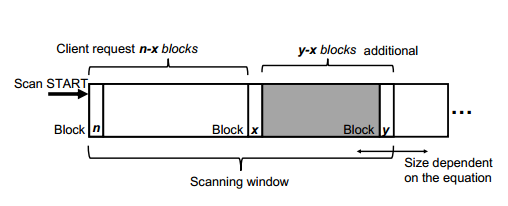
\includegraphics[width=0.7\linewidth]{image/Scanning_Window}
	\caption[پنجره پویش (\lr{Scanning Window}) ]{پنجره پویش. مطابق با تعداد بلوک‌های درخواست داده شده ($x$) و تعداد تراکنش‌های منطبق شده با درخواست مشتری در آن‌ها، احتمالا بلوک‌های بیشتری ($y$) از حافظه خوانده می‌شود تا نسبت بین بلوک‌های خوانده شده و اندازه پاسخ ثابت بماند\cite{Matetic2019}.}
	\label{fig:scanningwindow}
\end{figure}

روش دوم ارائه شده در \cite{Matetic2019} پایگاه داده ناآگاهانه نام دارد. در این روش کاربر سبک آدرس‌های مورد نظر خودش را، از طریق یک کانال محرمانه، برای SGX ارسال می‌کند و مستقیما اطلاعات مربوط به خروجی‌های خرج نشده را دریافت می‌نماید. در این روش برخلاف روش‌های پیشین و همچنین روش پنجره پویش،‌ نیاز نیست که کاربر سبک سرایند بلوک‌ها و مسیر (اثبات) درخت مرکل را دریافت و بررسی کند. در این روش کاربر به صحت عملکرد SGX و پاسخ آن اعتماد کامل دارد.
برای آنکه SGX بتواند کاربر را از صحت عملکرد خودش مطمئن سازد، 
تمام اقدامات و مقداردهی‌های اولیه به عنوان حالت اولیه ثبت می‌شود. با استفاده از آن کاربر می‌تواند مطمئن شود که کد صحیحی بر روی سامانه در حال اجرا است. به این فرایند تصدیق از راه دور\RTLfootnote{\lr{Remote Attestation}}
گفته می‌شود. تصدیق ایجاد شده، که شامل حالت اولیه است، امضا شده و برای کاربر ارسال می‌شود. کاربر می‌تواند توسط سرویس تصدیق برخطی که توسط اینتل ارائه می‌شود \cite{EPID}، امضا را بررسی نماید.

در روش پایگاه داده ناآگاهانه، SGX اطلاعات مربوط به خروجی خرج نشدهٔ تراکنش‌ها (UTXO) را در یک پایگاه داده رمزنگاری شده نگهداری می‌کند. همچنین از ماشین دسترسی تصادفی ناآگاهانهٔ
( ORAM\RTLfootnote{\lr{Oblivious Random Access Machine}})
معرفی شده در \cite{Stefanov2013} برای جلوگیری از نشت اطلاعات در هنگام دسترسی به حافظه استفاده می‌کند. به این ترتیب گره کامل متخاصم نمی‌تواند الگویی از دسترسی SGX به حافظه پیدا نماید. از طرف دیگر در این روش طول درخواست‌ها و پاسخ‌ها همواره یک مقدار ثابت است. اگر اندازه آن‌ها از آن مقدار ثابت کوتاه‌تر باشد، با لایی‌گذاری و اگر طولانی‌تر بود با تکه‌تکه کردن، به اندازه‌های ثابت تبدیل می‌شوند. در این روش SGX به تمام زنجیره بلوکی دسترسی ندارد و تنها دادهٔ UTXO را نگهداری کرده و به ازای اضافه شدن هر بلوک جدید، بعد از آن که آن بلوک را از جنبه اثبات کار و درخت مرکل درستی سنجی کرد، آن را به روزرسانی می‌کند. از آن‌جایی که UTXO در حافظه ORAM ذخیره می‌گردد، به روزرسانی آن امری نسبتا زمان‌بر، چیزی در حدود $78.5$ ثانیه، خواهد بود.

در دو روش ارائه شده در \cite{Matetic2019} بار پردازشی چندانی بر روی گره سبک قرار نخواهد گرفت. همچنین از آن‌جایی که دیگر لازم نیست برای حفظ حریم خصوصی کاربر تراکنش‌هایی مازاد به خاطر خطای نوع دو نیز دریافت شوند، پهنای باند به طور قابل ملاحظه‌ای در این دو روش نسبت به روش فیلتر بلوم کاهش پیدا می‌کند. از طرف دیگر در روش دوم (پایگاه داده ناآگاهانه) نیاز نیست که پاسخ گره کامل با اثبات‌های مرکل همراه باشد و به عبارتی گره سبک به عملکرد صحیح SGX اعتماد دارد. در نتیجه در این روش پهنای باند مصرفی بسیار کاهش پیدا می‌کند. علاوه بر مزایای ذکر شده، این روش ایراداتی نیز دارد که در ادامه به بیان آن خواهیم پرداخت.

اول از همه آنکه زمان تولید جواب در روش پنجره پویش، در صورتی که اقدامت مورد نیاز جهت جبران حمله کانال جانبی انجام شود، بسیار زمان‌بر است. به عنوان مثال برای پردازش  $100$ بلوک در این روش چیزی در حدود $73$ ثانیه زمان نیاز است. این زمان برای روش فیلتر بلوم با نرخ خطای نوع دوی $0.5$ درصد، حدود $1.1$ ثانیه است \cite{Matetic2019}. هر چند که تولید پاسخ در روش  پایگاه داده ناآگاهانه بسیار سریع‌تر انجام می‌شود، اما برای به روز رسانی داده خروجی‌ خرج نشده تراکنش‌ها نیاز به $78.5$ ثانیه زمان دارد. به عبارتی می‌توان اینطور گفت که هر ده دقیقه یک‌بار (زمان مورد نیاز برای استخراج یک بلوک جدید)، حدود یک دقیقه و هجده ثانیه،‌ صرف به روز رسانی شده و امکان پاسخ‌گویی به کاربران سبک را ندارد. مقاله \cite{Matetic2019} برای افزایش دسترس‌پذیری سیستم در شرایط به روز رسانی، پیشنهاد استفاده از دو سیستم موازی را داده است. در این شرایط نیز،‌ سیستم ارائه دهنده خدمات از وضعیت فعلی شبکه حداکثر حدود $78.5$ ثانیه عقب‌تر خواهد بود.

مشکل دیگری که روش \cite{Matetic2019} دارد، حملات فیزیکی کانال جانبی مدرنی است که SGX نسبت به آن‌ها آسیب‌پذیر است. مثلا حملات اسپکتر\RTLfootnote{\lr{Spectre}}\cite{Kocher2019}، ملت‌داون\RTLfootnote{\lr{Meltdown}}\cite{Lipp2020} و حمله \cite{Bulck2020} که به تازگی کشف شده است، می‌توانند برای استخراج کلید‌های تصدیق از ‌SGX مورد استفاده قرار گیرند. در صورتی که گره کامل متخاصم از چنین حمله‌ای بهره‌بردای کند، می‌تواند در روش پنجره پویش، حریم خصوصی کاربران سبک درخواست دهنده را نقض نماید؛ همچنین در روش پایگاه دادهٔ ناآگاهانه علاوه بر نقض حریم خصوصی کاربر سبک می‌تواند اطلاعات اشتباهی را در اختیار وی قرار دهد.

علاوه بر مشکلات ذکر شده در بالا، می‌توان به این مسئله نیز اشاره نمود که برای آنکه یک گره کامل بخواهد خدمات پیشنهاد شده در \cite{Matetic2019} را به گره‌های سبک ارائه دهد، نه تنها نیاز است که یک محیط اجرای قابل اطمینان تهیه و راه‌اندازی نماید، بلکه لازم است که منابع پردازشی قابل توجهی را برای این منظور اختصاص دهد. در نتیجه گره‌های کاملی که بتوانند چنین خدماتی ارائه دهند، محدود خواهند بود. به تبع آن کاربران سبک مجبور خواهند بود که بین گره‌های کامل محدود‌تری انتخاب کنند که این مسئله انگیزه این گره‌های کامل را برای انجام اقدامات خصمانه بیشتر خواهد کرد. از این اقدامات می‌توان به ایجاد و دنبال کردن یک انشعاب ناصحیح از زنجیره بلوکی بیت‌کوین اشاره نمود. در حالت عادی که تعداد گره‌های کامل زیاد هستند، گره سبک می‌تواند با دریافت خدمات از گره‌های کامل متعدد از صحت اطلاعات دریافتی مطمئن گردد.

از طرف دیگر، شرکت‌های محدودی مانند اینتل، تجهیزات مربوط به یک محیط اجرای قابل اطمینان را تولید و به فروش می‌رسانند. همچنین نیاز است که برای  تصدیق از راه دور عملکرد آن‌ها به سرویس‌هایی مثل \cite{EPID} وابسته بود. به بیان دیگر می‌توان این طور گفت که برای آنکه بتوان از روش \cite{Matetic2019} بهره‌برداری کرد، لازم است به شرکت‌های محدودی اعتماد شود که این خود بر خلاف ذات شبکه‌های همتابه‌همتایی مثل بیت کوین است.



\section{مقایسه}

در این فصل، ضمن آشنایی با ساز و کار فعلی شبکه‌ٔ همتا‌به‌همتای بیت‌کوین در ارسال اطلاعات مربوط به تراکنش‌های یک گره سبک با هدف حفظ حریم خصوصی وی \cite{Hearn2013}، توضیح داده شد که روش فعلی بسیار آسیب‌پذیر است و در صورتی که کاربر سبک خود اقداماتی را جهت حفظ بیشتر حریم خصوصیش انجام ندهد، عملا حریم خصوصی وی اصلا حفظ نمی‌شود.

علاوه بر این، در این فصل به بیان مفصل راه‌حل‌هایی که تا کنون برای رفع این مشکل ارائه شده‌اند، پرداخته شده است. در این قسمت این راه‌حل‌ها از سه جنبهٔ امنیت، پهنای باند مصرفی، بار پردازشی سمت گره کامل با هم مقایسه می‌شوند. که نتیجهٔ این مقایسه در جدول‌های زیر آورده شده است.

\begin{xltabular}{\textwidth}{|r|X|}
	\caption{
		مقایسهٔ امنیت روش‌های بحث شده.
		\label{table:SecurityCmp}}\\
	\hline
	\textbf{روش} & \textbf{آسیب‌پذیری‌ها} \\
	\hline 
	{%
		فیلتر بلوم \cite{Hearn2013}
	} & {%
		نرخ خطای نوع دوی عملا خیلی پایین، دسترسی به چند فیلتر بلوم از یک کاربر، کشف اولین استفاده از آدرس، تحلیل گراف تراکنش‌ها و کشف آدرس‌های مرتبط، تحلیل بسامد استفاده از آدرس، تحلیل زمان درخواست
	} \\
\hline
	{%
		اصلاح رفتار گره سبک \cite{Gervais2014}
	} & {%
		کشف اولین استفاده از آدرس، تحلیل گراف تراکنش‌ها و کشف آدرس‌های مرتبط، تحلیل بسامد استفاده از آدرس، تحلیل زمان درخواست
	}\\
\hline
	{%
		معیار حاشاپذیری-$\gamma$ \cite{Kanemura2017}
	} & {%
		دسترسی به چند فیلتر بلوم از یک کاربر، کشف اولین استفاده از آدرس، تحلیل گراف تراکنش‌ها و کشف آدرس‌های مرتبط، تحلیل بسامد استفاده از آدرس، تحلیل زمان درخواست
	}\\
\hline
	{%
		فیلتر بلوک \cite{Osuntokun2017}
	} & {%
		تحلیل گراف تراکنش‌ها و کشف آدرس‌های مرتبط، تحلیل بسامد استفاده از آدرس، تحلیل زمان درخواست
	}\\
\hline
	{%
		بازیابی اطلاعات خصوصی \cite{Qin2019}
	} & {%
		تبانی گره‌های کامل، تحلیل زیردسته‌های دستهٔ تمام-مدت مورد پرسمان واقع شده، تحلیل بسامد استفاده در زیردسته‌ها، سخت بودن راه‌اندازی یک گره کامل در نتیجه نیاز به اعتماد به گره‌های اندک موجود
	}\\
\hline
	{%
		پنجرهٔ پویش (\lr{SGX}) \cite{Matetic2019}
	} & {%
		اعتماد به سازنده‌های سخت‌افزار محیط‌های قابل اعتماد، افشای اطلاعات در صورت حملات کانال جانبی، سخت بودن راه‌اندازی یک گره کامل در نتیجه نیاز به اعتماد به گره‌های اندک موجود
	}\\
\hline
	{%
		پایگاه دادهٔ ناآگاهانه (\lr{SGX}) \cite{Matetic2019}
	} & {%
		اعتماد به سازنده‌های سخت‌افزار محیط‌های قابل اعتماد، افشای اطلاعات در صورت حملات کانال جانبی، ارسال اطلاعات نادرست در صورت حملات کانال جانبی، سخت بودن راه‌اندازی یک گره کامل در نتیجه نیاز به اعتماد به گره‌های اندک موجود
	}\\
\hline	
\end{xltabular}

\begin{xltabular}{\textwidth}{|r|X|}
	\caption{
		مقایسهٔ پهنای باند مصرفی در روش‌های بحث شده.
		\label{table:BandWidthCmp}}\\
	\hline
	\textbf{روش} & \textbf{پهنای باند} \\
	\hline 
	{%
		فیلتر بلوم \cite{Hearn2013}
	} & {%
		به خاطر به‌روز رسانی فیلتر توسط گره کامل، از خیلی کم به زیاد تغییر می‌کند. شامل تراکنش‌ها و اثبات مرکل
	} \\
	\hline
	{%
		اصلاح رفتار گره سبک \cite{Gervais2014}
	} & {%
		متوسط - نرخ خطای نوع دو بالاتر از روش \cite{Hearn2013}. شامل تراکنش‌ها و اثبات مرکل.
	}\\
	\hline
	{%
		معیار حاشاپذیری-$\gamma$ \cite{Kanemura2017}
	} & {%
		کم
	}\\
	\hline
	{%
		فیلتر بلوک \cite{Osuntokun2017}
	} & {%
		برای گره‌های مختلف با تعداد تراکنش‌های مختلف متفاوت است.
	}\\
	\hline
	{%
		بازیابی اطلاعات خصوصی \cite{Qin2019}
	} & {%
		خیلی زیاد. اندازهٔ فایل مانیفست تمام-مدت $3.30$ گیگابایت
	}\\
	\hline
	{%
		پنجرهٔ پویش (\lr{SGX}) \cite{Matetic2019}
	} & {%
		خیلی کم. شامل تراکنش‌های مرتبط و اثبات مرکل. بدون خطای نوع دو.
	}\\
	\hline
	{%
		پایگاه دادهٔ ناآگاهانه (\lr{SGX}) \cite{Matetic2019}
	} & {%
		ناچیز. شامل تراکنش‌های مرتبط بدون نیاز به اثبات مرکل و بدون خطای نوع دو.
	}\\
	\hline	
\end{xltabular}

\begin{xltabular}{\textwidth}{|r|X|}
	\caption{
		مقایسهٔ پردازش سمت گره کامل در روش‌های بحث شده.
		\label{table:ProcCmp}}\\
	\hline
	\textbf{روش} & \textbf{پهنای باند} \\
	\hline 
	{%
		فیلتر بلوم \cite{Hearn2013}
	} & {%
		زیاد - برای هر فیلتر بلوم باید چیکدهٔ تمام داده‌های تراکنش‌های یک بلوک $k$ بار حساب شود. 
	} \\
	\hline
	{%
		اصلاح رفتار گره سبک \cite{Gervais2014}
	} & {%
		زیاد - برای هر فیلتر بلوم باید چیکدهٔ تمام داده‌های تراکنش‌های یک بلوک $k$ بار حساب شود.
	}\\
	\hline
	{%
		معیار حاشاپذیری-$\gamma$ \cite{Kanemura2017}
	} & {%
		زیاد - برای هر فیلتر بلوم باید چیکدهٔ تمام داده‌های تراکنش‌های یک بلوک $k$ بار حساب شود.
	}\\
	\hline
	{%
		فیلتر بلوک \cite{Osuntokun2017}
	} & {%
		کم - فقط یک بار باید چکیدهٔ تمام داده‌های تراکنش‌های یک بلوک حساب شده و برای فشرده‌سازی، کدگذاری شوند.
	}\\
	\hline
	{%
		بازیابی اطلاعات خصوصی \cite{Qin2019}
	} & {%
		زیاد. به ازای استخراج یک بلوک جدید باید دستهٔ هفتگی به روز رسانی شود.
	}\\
	\hline
	{%
		پنجرهٔ پویش (\lr{SGX}) \cite{Matetic2019}
	} & {%
		خیلی خیلی زیاد. به ازای درخواست هر کاربر سبک باید تمام اثبات‌های مرکل تمام تراکنش‌های چند بلوک را حساب کند. تعداد بلوک‌های محاسبه شده با توجه به درخواست کاربر تعیین می‌شود.
	}\\
	\hline
	{%
		پایگاه دادهٔ ناآگاهانه (\lr{SGX}) \cite{Matetic2019}
	} & {%
		زیاد. به ازای استخراج هر بلوک جدید، باید پایگاه‌داده ناآگاهانه را به روزرسانی کند.
	}\\
	\hline	
\end{xltabular}